

\mode<presentation>
{
  \usetheme{boxes}
  %\useoutertheme{infolines}
  % með efnisyfirliti: Szeged, Frankfurt 
  % án efnisyfirlits: Pittsburgh
  % áhugavert: CambridgeUS, Boadilla
  %\setbeamercovered{transparent} %gegnsætt
  \setbeamercovered{invisible}

\defbeamertemplate*{footline}{infolines theme}
{
  \leavevmode%
  \hbox{%
  \begin{beamercolorbox}[wd=.333333\paperwidth,ht=2.25ex,dp=1ex,center]{author in head/foot}%
  %  \usebeamerfont{author in head/foot}\insertshortauthor~~\beamer@ifempty{\insertshortinstitute}{}{(\insertshortinstitute)}
  \end{beamercolorbox}%
  \begin{beamercolorbox}[wd=.333333\paperwidth,ht=2.25ex,dp=1ex,center]{title in head/foot}%
   % \usebeamerfont{title in head/foot}\insertshorttitle
  \end{beamercolorbox}%
  \begin{beamercolorbox}[wd=.333333\paperwidth,ht=2.25ex,dp=1ex,right]{date in head/foot}%
    %\usebeamerfont{date in head/foot}\insertshortdate{}\hspace*{2em}
    \insertshortlecture.\insertframenumber{} / \insertshortlecture.\inserttotalframenumber\hspace*{2ex} 
  \end{beamercolorbox}}%
  \vskip0pt%
}
\resetcounteronoverlays{rtaskno} %Does not increase counter rtaskno on \pause in beamer


}


\usepackage[english,icelandic]{babel}
\usepackage[utf8]{inputenc}
\usepackage{t1enc}
\usepackage{graphicx}
\usepackage{amsmath}
\usepackage{amssymb}
\usepackage{mathrsfs}
\usepackage{verbatim}
\usepackage{esint}


% RAGNAR SIGURÐSSON
%\usepackage[T1]{fontenc} 
%\usepackage[icelandic]{babel}
\usepackage{latexsym,amssymb,amsmath}
%\usepackage[utf8]{inputenc}
%\usepackage{graphicx}
\usepackage{epstopdf}
\usepackage{verbatim}
\usepackage{array,tabularx,arydshln}
\setbeamertemplate{theorems}[numbered]


\newtheorem{setning}{Setning}
\newtheorem{hjalpar}{Hjálparsetning}
\theoremstyle{definition}
\newtheorem{rithattur}{Ritháttur}
\newtheorem{skilgreining}{Skilgreining}
\newtheorem{daemi}{Dæmi}
\newtheorem{ath}{Athugasemd}

\newcommand\Wider[2][3em]{%
\makebox[\linewidth][c]{%
  \begin{minipage}{\dimexpr\textwidth+#1\relax}
  \raggedright#2
  \end{minipage}%
  }%
}

%counter used for blocks
\newcounter{rtaskno}
\DeclareRobustCommand{\rtask}[1]{%
   \refstepcounter{rtaskno}%
   \thertaskno\label{#1}}

\newcommand{\C}{{\mathbb  C}}
\newcommand{\Z}{{\mathbb Z}}
\newcommand{\R}{{\mathbb  R}}
\newcommand{\N}{{\mathbb  N}}
\newcommand{\Q}{{\mathbb Q}}
\renewcommand{\phi}{\varphi}
\renewcommand{\epsilon}{\varepsilon}
\newcommand{\p}{{\partial}}
\renewcommand{\d}{{\partial}}

% RAGNAR SIGURÐSSON
\newcommand{\nin}{\mbox{$\;\not\in\;$}}
\newcommand{\dive}{\mbox{${\rm\bf div\,}$}}
\newcommand{\curl}{\mbox{${\rm\bf curl\,}$}}
\newcommand{\grad}{\mbox{${\rm\bf grad\,}$}}
\newcommand{\spann}{\mbox{${\rm Span}$}}
\newcommand{\tr}{\mbox{${\rm tr}$}}
\newcommand{\rank}{\mbox{${\rm rank}$}}
\newcommand{\image}{\mbox{${\rm image}$}}
\newcommand{\nullity}{\mbox{${\rm null}$}}
\newcommand{\proj}{\mbox{${\rm proj}$}}
\newcommand{\id}{\mbox{${\rm id}$}}
%\newcommand{\R}{\mbox{${\bf R}$}}
%\newcommand{\C}{\mbox{${\bf C}$}}
\newcommand{\Rn}{\mbox{${\bf R}^n$}}
\newcommand{\Rm}{\mbox{${\bf R}^m$}}
\newcommand{\Rk}{\mbox{${\bf R}^k$}}
\newcommand{\Av}{\mbox{${\bf A}$}}
\newcommand{\av}{\mbox{${\bf a}$}}
\newcommand{\uv}{\mbox{${\bf u}$}}
\newcommand{\vv}{\mbox{${\bf v}$}}
\newcommand{\wv}{\mbox{${\bf w}$}}
\newcommand{\xv}{\mbox{${\bf x}$}}
\newcommand{\zv}{\mbox{${\bf z}$}}
\newcommand{\yv}{\mbox{${\bf y}$}}
\newcommand{\bv}{\mbox{${\bf b}$}}
\newcommand{\cv}{\mbox{${\bf c}$}}
\newcommand{\dv}{\mbox{${\bf d}$}}
\newcommand{\ev}{\mbox{${\bf e}$}}
\newcommand{\fv}{\mbox{${\bf f}$}}
\newcommand{\gv}{\mbox{${\bf g}$}}
\newcommand{\hv}{\mbox{${\bf h}$}}
\newcommand{\iv}{\mbox{${\bf i}$}}
\newcommand{\jv}{\mbox{${\bf j}$}}
\newcommand{\kv}{\mbox{${\bf k}$}}
\newcommand{\pv}{\mbox{${\bf p}$}}
\newcommand{\nv}{\mbox{${\bf n}$}}
\newcommand{\qv}{\mbox{${\bf q}$}}
\newcommand{\rv}{\mbox{${\bf r}$}}
\newcommand{\sv}{\mbox{${\bf s}$}}
\newcommand{\tv}{\mbox{${\bf t}$}}
\newcommand{\ov}{\mbox{${\bf 0}$}}
\newcommand{\Fv}{\mbox{${\bf F}$}}
\newcommand{\Gv}{\mbox{${\bf G}$}}
\newcommand{\Uv}{\mbox{${\bf U}$}}
\newcommand{\Nv}{\mbox{${\bf N}$}}
\newcommand{\Hv}{\mbox{${\bf H}$}}
\newcommand{\Ev}{\mbox{${\bf E}$}}
\newcommand{\Sv}{\mbox{${\bf S}$}}
\newcommand{\Tv}{\mbox{${\bf T}$}}
\newcommand{\Bv}{\mbox{${\bf B}$}}
\newcommand{\Oa}{\mbox{$(0,0)$}}
\newcommand{\Ob}{\mbox{$(0,0,0)$}}
\newcommand{\Onv}{\mbox{$[0,0,\ldots,0]$}}
\newcommand{\an}{\mbox{$(a_1,a_2, \ldots,a_n)$}}
\newcommand{\xn}{\mbox{$(x_1,x_2, \ldots,x_n)$}}
\newcommand{\xnv}{\mbox{$[x_1,x_2, \ldots,x_n]$}}
\newcommand{\vnv}{\mbox{$[v_1,v_2, \ldots,v_n]$}}
\newcommand{\wnv}{\mbox{$[w_1,w_2, \ldots,w_n]$}}
\newcommand{\tvint}{\int\!\!\!\int}
\newcommand{\thrint}{\int\!\!\!\int\!\!\!\int}
\renewcommand{\ast}{{\operatorname{\text{astand}}}}


\usepackage{caption}
%\usepackage{pgfpages}
% \pgfpagesuselayout{2 on 1}[a4paper,border shrink=5mm]

\def\lecturename{Stærðfræðigreining IIB}
\title{\insertlecture}
\author{Sigurður Örn Stefánsson, \href{mailto:sigurdur@hi.is}{sigurdur@hi.is}}
\institute
{
  Verkfræði- og náttúruvísindasvið\\
  Háskóli Íslands
}
\subtitle{Stærðfræðigreining IIB, STÆ205G}
%\subject{\lecturename}

\mode<article>
{
	\usepackage[colorlinks=false,
	pdfauthor={Sigurður Örn Stefánson},
	%pdftitle={Töluleg greining}
	]{hyperref}
  %\usepackage{times}
  %\usepackage{mathptmx}
  \usepackage[left=1.5cm,right=4cm,top=1.5cm,bottom=3cm]{geometry}
}

% Beamer version theme settings

%\useoutertheme[height=0pt,width=2cm,right]{sidebar}
%\usecolortheme{rose,sidebartab}
%\useinnertheme{circles}
%\usefonttheme[only large]{structurebold}


\setbeamercolor{sidebar right}{bg=black!15}
\setbeamercolor{structure}{fg=blue}
\setbeamercolor{author}{parent=structure}

\setbeamerfont{title}{series=\normalfont,size=\LARGE}
\setbeamerfont{title in sidebar}{series=\bfseries}
\setbeamerfont{author in sidebar}{series=\bfseries}
\setbeamerfont*{item}{series=}
\setbeamerfont{frametitle}{size=}
\setbeamerfont{block title}{size=\small}
\setbeamerfont{subtitle}{size=\normalsize,series=\normalfont}


\setbeamertemplate{sidebar right}
{
  {\usebeamerfont{title in sidebar}%
    \vskip1.5em%
    \hskip3pt%
    \usebeamercolor[fg]{title in sidebar}%
    \insertshorttitle[width=2cm-6pt,center,respectlinebreaks]\par%
    \vskip1.25em%
  }%
  {%
    \hskip3pt%
    \usebeamercolor[fg]{author in sidebar}%
    \usebeamerfont{author in sidebar}%
    \insertshortauthor[width=2cm-2pt,center,respectlinebreaks]\par%
    \vskip1.25em%
  }%
  \hbox to2cm{\hss\insertlogo\hss}
  \vskip1.25em%
  \insertverticalnavigation{2cm}%
  \vfill
  \hbox to 2cm{\hfill\usebeamerfont{subsection in
      sidebar}\strut\usebeamercolor[fg]{subsection in
      sidebar}\insertshortlecture.\insertframenumber\hskip5pt}%
  \vskip3pt%
}%

\setbeamertemplate{title page}
{
  \vbox{}
  \vskip1em
  %{\huge Kapitel \insertshortlecture\par}
  {\usebeamercolor[fg]{title}\usebeamerfont{title}\inserttitle\par}%
  \ifx\insertsubtitle\@empty%
  \else%
    \vskip0.25em%
    {\usebeamerfont{subtitle}\usebeamercolor[fg]{subtitle}\insertsubtitle\par}%
  \fi%     
  \vskip1em\par
  %Vorlesung \emph{\lecturename}\ vom 
  \insertdate\par
  \vskip0pt plus1filll
  \leftskip=0pt plus1fill\insertauthor\par
  \insertinstitute\vskip1em
}

%\logo{\includegraphics[width=2cm]{beamerexample-lecture-logo.pdf}}



% Article version layout settings

\mode<article>

\makeatletter
\def\@listI{\leftmargin\leftmargini
  \parsep 0pt
  \topsep 5\p@   \@plus3\p@ \@minus5\p@
  \itemsep0pt}
\let\@listi=\@listI


\setbeamertemplate{frametitle}{\paragraph*{\insertframetitle\
    \ \small\insertframesubtitle}\ \par
}
\setbeamertemplate{frame end}{%
  \marginpar{\scriptsize\hbox to 1cm{\sffamily%
      \hfill\strut\insertshortlecture.\insertframenumber}\hrule height .2pt}}
\setlength{\marginparwidth}{1cm}
\setlength{\marginparsep}{1.5cm}

\def\@maketitle{\makechapter}

\def\makechapter{
  \newpage
  \null
  \vskip 2em%
  {%
    \parindent=0pt
    \raggedright
    \sffamily
    \vskip8pt
    %{\fontsize{36pt}{36pt}\selectfont Kapitel \insertshortlecture \par\vskip2pt}
    {\fontsize{24pt}{28pt}\selectfont \color{blue!50!black} \insertlecture\par\vskip4pt}
    {\Large\selectfont \color{blue!50!black} \insertsubtitle, \@date\par}
    \vskip10pt

    \normalsize\selectfont \@author\par\vskip1.5em
    %\hfill BLABLA
  }
  \par
  \vskip 1.5em%
}

\let\origstartsection=\@startsection
\def\@startsection#1#2#3#4#5#6{%
  \origstartsection{#1}{#2}{#3}{#4}{#5}{#6\normalfont\sffamily\color{blue!50!black}\selectfont}}

\makeatother

\mode
<all>



% Typesetting Listings

\usepackage{listings}
\lstset{language=Java}

\alt<presentation>
{\lstset{%
  basicstyle=\footnotesize\ttfamily,
  commentstyle=\slshape\color{green!50!black},
  keywordstyle=\bfseries\color{blue!50!black},
  identifierstyle=\color{blue},
  stringstyle=\color{orange},
  escapechar=\#,
  emphstyle=\color{red}}
}
{
  \lstset{%
    basicstyle=\ttfamily,
    keywordstyle=\bfseries,
    commentstyle=\itshape,
    escapechar=\#,
    emphstyle=\bfseries\color{red}
  }
}



% Common theorem-like environments

\theoremstyle{definition}
\newtheorem{exercise}[theorem]{\translate{Exercise}}




% New useful definitions:

\newbox\mytempbox
\newdimen\mytempdimen

\newcommand\includegraphicscopyright[3][]{%
  \leavevmode\vbox{\vskip3pt\raggedright\setbox\mytempbox=\hbox{\includegraphics[#1]{#2}}%
    \mytempdimen=\wd\mytempbox\box\mytempbox\par\vskip1pt%
    \fontsize{3}{3.5}\selectfont{\color{black!25}{\vbox{\hsize=\mytempdimen#3}}}\vskip3pt%
}}

\newenvironment{colortabular}[1]{\medskip\rowcolors[]{1}{blue!20}{blue!10}\tabular{#1}\rowcolor{blue!40}}{\endtabular\medskip}

\def\equad{\leavevmode\hbox{}\quad}

\newenvironment{greencolortabular}[1]
{\medskip\rowcolors[]{1}{green!50!black!20}{green!50!black!10}%
  \tabular{#1}\rowcolor{green!50!black!40}}%
{\endtabular\medskip}


\begin{document}

\section{Vigursvið}

\subsection{Vigursvið} 

\subsubsection{Skilgreining }
 {\em Vigursvið} á $\R^2$ er vörpun
$$\Fv(x,y)=F_1(x,y)\,\iv+F_2(x,y)\,\jv.$$
Þegar talað er um vigursvið þá hugsum við vigurinn $\Fv(x,y)$ sem vigur í
$\R^2$ sem hefur fótpunkt í punktinum $(x,y)$.   

 \medskip
Vigursvið $\Fv(x,y)=F_1(x,y)\iv+F_2(x,y)\jv$ er sagt {\em samfellt} ef
föllin $F_1(x,y)$ og $F_2(x,y)$ eru samfelld.

\medskip
Vigursvið á $\R^3$ er vörpun 
$$\Fv(x,y,z)=F_1(x,y,z)\,\iv+F_2(x,y,z)\,\jv+F_3(x,y,z)\,\kv.$$
Við hugsum $\Fv(x,y,z)$ sem vigur með $(x,y,z)$ sem fótpunkt.
  Skilgreiningin á því að
vigursvið í $\R^3$ sé samfellt er eins og á samfeldni vigursvið í
$\R^2$ . 



 \begin {figure}[h!]
 \centering
            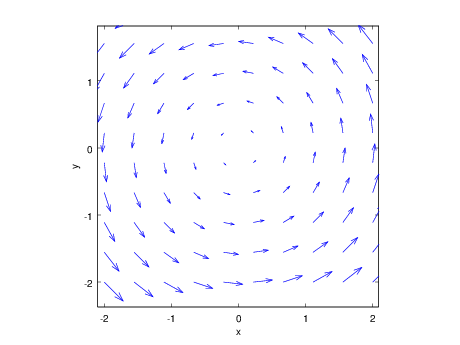
\includegraphics[width=0.75\linewidth]{vfield.png}
            \caption*{ Vigursviðið $\mathbf{F}(x,y) = -y\iv + x \jv$.}
\end {figure}






\subsection{Straumlína} 

\subsubsection{Skilgreining }
 Ferill $C$ í planinu kallast {\em straumlína}
(e.~stream line, flow line)
fyrir vigursvið $\Fv(x,y)$ ef í hverjum punkti $(x,y)$ á ferlinum er
vigurinn $\Fv(x,y)$ snertivigur við ferilinn. 


 \begin {figure}[h!]
 \centering
            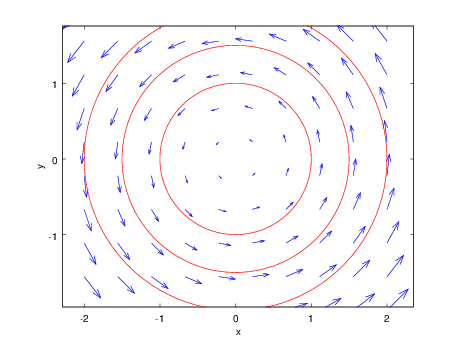
\includegraphics[width=0.55\linewidth]{flowlines.png}
            \caption*{Vigursviðið $\mathbf{F}(x,y) = -y\iv + x \jv$ ásamt nokkrum straumlínum.}
\end {figure}




\subsection{Stigulsvið} 

\subsubsection{Skilgreining }
Vigursvið $\Fv(x,y)$ kallast {\em stigulsvið} eða {\em geymið svið}
(e.~gradient field, conservative  field) á mengi $D$ ef til er fall $\phi(x,y)$ þannig að $$\Fv(x,y)=\nabla\phi(x,y)$$ fyrir alla punkta $(x,y)\in D$, það er að segja ef 
$$\Fv(x,y)=F_1(x,y)\,\iv+F_2(x,y)\,\jv$$ 

þá er $$F_1(x,y)=\frac{\partial}{\partial x}\phi(x,y) \quad \text{og}\quad  F_2(x,y)=\frac{\partial}{\partial y}\phi(x,y).$$

Vigursvið $\Fv(x,y,z)$ kallast {\em stigulsvið} eða  {\em geymið svið} ef til er fall $\phi(x,y,z)$ þannig að $\Fv(x,y,z)=\nabla\phi(x,y,z)$. 

\medskip
Fallið $\phi$ kallast {\em mætti} (e.~potential) fyrir vigursviðið $\Fv$.



\subsubsection{Setning }
 Látum $\Fv(x,y)=F_1(x,y)\,\iv+F_2(x,y)\,\jv$ vera vigursvið þannig að föllin $F_1(x,y)$ og $F_2(x,y)$ hafi samfelldar hlutafleiður.  Ef $\Fv(x,y)$ er stigulsvið þá er 
$$\frac{\partial}{\partial y}F_1(x,y)=
\frac{\partial}{\partial x}F_2(x,y).$$

\smallskip

{\bf Athugasemd.}  Þó að hlutafleiðurnar séu jafnar
þá er {\bf ekki} hægt að álykta að $\Fv$ sé stigulsvið.  Þetta
atriði verður rætt síðar.
 



\subsubsection{Setning }
Látum
$\Fv(x,y,z)=F_1(x,y,z)\,\iv+F_2(x,y,z)\,\jv+F_3(x,y,z)\,\kv$ vera vigursvið
þannig að föllin $F_1(x,y,z), F_2(x,y,z)$ og $F_3(x,y,3)$ hafi
samfelldar hlutafleiður.  Ef $\Fv(x,y,z)$ er stigulsvið þá er  

\begin {align*}
\frac{\partial}{\partial y}F_1(x,y,z) &=
\frac{\partial}{\partial x}F_2(x,y,z), \\
\frac{\partial}{\partial z}F_1(x,y,z) &=
\frac{\partial}{\partial x}F_3(x,y,z) \quad \text{og} \\
\frac{\partial}{\partial z}F_2(x,y,z)&=
\frac{\partial}{\partial y}F_3(x,y,z).
\end {align*}





\subsubsection{Reikniaðferð }
 Finna á mætti $\phi(x,y)$ fyrir stigulsvið  $\Fv(x,y)=F_1(x,y)\,\iv+F_2(x,y)\,\jv$.  Viljum finna fall $\phi(x,y)$ þannig að 
$$\frac{\partial}{\partial x}\phi(x,y)=F_1(x,y)\qquad
\mbox{og}\qquad \frac{\partial}{\partial y}\phi(x,y)=F_2(x,y).$$
 Með því að heilda þessar jöfnur fæst að 
 $$\phi(x,y)=\int F_1(x,y)\,dx+C_1(y)$$
og
$$\phi(x,y)=\int F_2(x,y)\,dy+C_2(x).$$

Þegar fyrra stofnfallið er reiknað þá er $y$ hugsað sem fasti og því fæst heildunarfasti sem getur verið fall af $y$.  Lokaskrefið er  svo að horfa á jöfnurnar tvær hér að ofan og sjá hvort ekki er hægt að finna gildi fyrir heildunarfastanna $C_1(x)$ og $C_2(y)$ þannig að sama formúlan fyrir $\phi(x,y)$ fáist.  



\subsection{Heildi falls yfir feril} 

\subsubsection{Skilgreining }
Látum $\cal C$ vera feril í $\R^2$ stikaðan af samfellt diffranlegum stikaferli $\rv:[a,b]\rightarrow\R^2$.  Ritum $\rv(t)=(x(t),y(t))$.  {\em Heildi falls} $f(x,y)$ {\em yfir ferilinn} $\cal C$ {\em með tilliti til bogalengdar} er skilgreint sem 
\begin{align*}  
\int_{\cal C}f(x,y)\,ds&=\int_a^b f(\rv(t))\,|\rv'(t)|\,dt\\
&=\int_a^b f(x(t),y(t))\,\sqrt{x'(t)^2+y'(t)^2}\,dt.\end{align*}
Sama aðferð notuð til að skilgreina heildi falls yfir feril í $\R^3$.



\subsubsection{Setning }
 Látum $\cal C$ vera feril í $\R^2$.  Gerum ráð fyrir að $\rv_1$ og $\rv_2$ séu tveir samfellt diffranlegir stikaferlar sem báðir stika ferilinn $\cal C$.  Ef fall $f(x,y)$ er heildað yfir $\cal C$ þá fæst sama útkoma hvort sem stikunin $\rv_1$ eða stikunin $\rv_2$ er notuð við útreikningana.




\subsubsection{Skilgreining }
Ferill $\cal C$ í plani er sagður {\em samfellt diffranlegur á köflum} ef til er stikun $\rv:[a,b]\rightarrow \R^2$ á $\cal C$ þannig að  til eru punktar $a=t_0<t_1<t_2<\cdots<t_n<t_{n+1}=b$ þannig að á hverju bili $(t_i,t_{i+1})$ er $\rv$ samfellt diffranlegur ferill og markgildin
$$\lim_{t\rightarrow t_i^+}\rv'(t)\qquad\mbox{og}\qquad 
\lim_{t\rightarrow t_{i+1}^-}\rv'(t)$$
eru bæði til.  

Líka sagt að stikaferillinn $\rv$ sé {\em samfellt diffranlegur á köflum.}



\subsection{Heildi vigursviðs eftir ferli} 

\subsubsection{Skilgreining }
Látum $\Fv(x,y)$ vera vigursvið og $\rv:[a,b]\rightarrow \R^2$ stikun á ferli $\cal C$ og gerum ráð fyrir að stikaferillinn $\rv$ sé samfellt diffranlegur á köflum.  {\em Heildi vigursviðsins} $\Fv(x,y)$ {\em eftir ferlinum} $\cal C$ er skilgreint sem 
$$\int_{\cal C} \Fv\cdot d\rv= \int_{\cal C} \Fv\cdot \Tv\,ds
=\int_a^b \Fv(\rv(t))\cdot \rv'(t)\,dt.$$



\subsubsection{Skilgreining }
Ritum $\Fv(x,y)=F_1(x,y)\,\iv+F_2(x,y)\,\jv$.  Ritum líka $\rv(t)=x(t)\,\iv+y(t)\,\jv$.  Þá má rita
$dx=x'(t)\,dt,\, dy=y'(t)\,dt$.  Með því að nota þennan rithátt fæst að 
\begin{align*}
\int_{\cal C}\Fv\cdot d\rv&=\int_a^b
(F_1(x,y)\,\iv+F_2(x(t),y(t))\,\jv)\cdot(x'(t)\,\iv+y'(t)\,\jv)\,dt\\
&=\int_a^b F_1(x(t),y(t))x'(t)\,dt+F_2(x(t),y(t))y'(t)\,dt\\
&=\int_{\cal C} F_1(x,y)\,dx+F_2(x,y)\,dy.
\end{align*}




\subsubsection{Athugasemd }
Látum $\cal C$ vera feril í $\R^2$. Gerum ráð fyrir að $\rv_1:[a,b]\rightarrow \R^2$ og  $\rv_2:[a',b']\rightarrow \R^2$ séu tveir samfellt diffranlegir á köflum stikaferlar sem stika $\cal C$.  Gerum ennfremur ráð fyrir að $\rv_1(a)=\rv_2(b')$ og $\rv_1(b)=\rv_2(a')$ (þ.e.a.s. stikaferlarnir fara í sitthvora áttina eftir $\cal C$).  Þá gildir ef $\Fv(x,y)$ er vigursvið að 
$$\int_{\cal C} \Fv\cdot d\rv_1=-\int_{\cal C} \Fv\cdot d\rv_2.$$
(Ef breytt er um stefnu á stikun á breytist formerki þegar vigursvið heildað eftir ferlinum.)





\subsection{Ferilheildi og stigulsvið} 

\subsubsection{Setning \rtask{}}
Látum $\Fv(x,y)$ vera samfellt stigulsvið skilgreint á svæði $D$ í $\R^2$ og látum $\phi$ vera fall skilgreint á $D$ þannig að $\Fv(x,y)=\nabla \phi(x,y)$ fyrir alla punkta $(x,y)\in D$.   Látum $\rv:[a,b]\rightarrow D$ vera stikaferill sem er samfellt diffranlegur á köflum og stikar feril $\cal C$ í $D$.  Þá er
$$\int_{\cal C} \Fv\cdot \,d\rv=\phi(\rv(b))-\phi(\rv(a)).$$
(Samsvarandi gildir fyrir vigursvið skilgreint á svæði $D\subseteq \R^3$.)






\subsubsection{Fylgisetning \rtask{}} %\label{thm:atob}}
Látum $\Fv$ vera samfellt stigulsvið
skilgreint á mengi $D\subseteq \R^2$.   Látum $\rv:[a,b]\rightarrow D$ vera
stikaferil sem er samfellt diffranlegur á köflum og lokaður (þ.e.a.s. $\rv(a)=\rv(b)$) og stikar feril $\mathcal{C}$.  Þá er $$\oint_{\cal C}  \Fv\cdot \,d\rv=0.$$

(Ath.~að rithátturinn $$\oint_{\cal C}$$ er gjarnan notaður þegar heildað er yfir lokaðan feril $\cal C$.)




\subsubsection{Fylgisetning \rtask{}}
Látum $\Fv$ vera samfellt stigulsvið
skilgreint á mengi $D\subseteq \R^2$.   Látum
$\rv_1:[a_1,b_1]\rightarrow D$ og $\rv_2:[a_2,b_2]\rightarrow D$ vera
stikaferla sem eru samfellt diffranlegir á köflum og stika ferlana $\mathcal{C}_1$ og $\mathcal{C}_2$.  Gerum ráð fyrir
að $\rv_1(a_1)=\rv_2(a_2)$ og $\rv_1(b_1)=\rv_2(b_2)$, þ.e.a.s.\ stikaferlarnir $\rv_1$ og $\rv_2$ hafa sameiginlega upphafs- og endapunkta.   Þá er  
$$\int_{{\cal C}_1} \Fv\cdot\,d\rv_1=\int_{{\cal C}_2} \Fv\cdot\,d\rv_2.$$ 
 


\subsubsection{Skilgreining \rtask{}}
 Segjum að heildi vigursviðs $\Fv$ sé {\em
  óháð stikaferli} ef fyrir sérhverja tvo samfellt diffranlega á
köflum stikaferla $\rv_1$ og $\rv_2$ með sameiginlega upphafs- og
endapunkta sem stika ferlana $\mathcal{C}_1$ og $\mathcal{C}_2$ gildir að  
$$\int_{{\cal C}_1} \Fv\cdot\,d\rv_1=
\int_{{\cal C}_2} \Fv\cdot\,d\rv_2.$$ 



\subsubsection{Setning \rtask{thm:beqc}}
  Ferilheildi samfellds vigursviðs $\Fv$ er óháð
stikaferli ef og aðeins ef $\oint_{\cal C} \Fv\cdot\,d\rv=0$ fyrir alla
lokaða ferla $\cal C$ sem eru samfellt diffranlegir á köflum. 



\subsubsection{Skilgreining \rtask{}}
   Segjum að mengi $D\subseteq \R^2$ sé {\em
  ferilsamanhangandi} (e. connected, path-connected)  ef fyrir
  sérhverja tvo punkta $P, Q\in D$ gildir 
að til er stikaferill $\rv:[0,1]\rightarrow D$ þannig að $\rv(0)=P$ og
$\rv(1)=Q$.

\bigskip
(Athugasemd:  Í bók er orðið {\em connected} notað fyrir hugtakið {\em
  ferilsamanhangandi}.  Venjulega er orðið {\em connected} notað yfir
  annað hugtak, skylt en samt ólíkt.)




\subsubsection{Setning \rtask{thm:ctoa} }
 Látum $D$ vera opið mengi í $\R^2$ sem er ferilsamanhangandi.  Ef $\Fv$ er samfellt vigursvið skilgreint á $D$ og ferilheildi $\Fv$ eru óháð vegi þá er $\Fv$ stigulsvið.
    



\subsubsection{Setning \rtask{}}
 Fyrir samfellt vigursvið $\Fv$ skilgreint á opnu 
ferilsamanhangandi mengi $D\subseteq \R^2$ er eftirfarandi jafngilt:
\begin{itemize}
 \item [(a)] $\Fv$ er stigulsvið,
 \item [(b)]  $\oint_{\cal C} \Fv\cdot\,d\rv=0$ fyrir alla samfellt diffranlega
á köflum lokaða stikaferla $\rv$ í $D$, 
\item [(c)] ferilheildi $\Fv$ er óháð vegi.
\end{itemize}

\pause
\subsubsection{Sönnun: } 
(a) $\Rightarrow$ (b). Fylgisetning \ref{thm:atob}. \\
(b) $\Leftrightarrow$ (c). Setning \ref{thm:beqc}. \\
(c) $\Rightarrow$ (a). Setning \ref{thm:ctoa}.
 




\subsection{Fletir} 

\subsubsection{Óformleg skilgreining  \rtask{}}
Flötur $\cal S$ í $\R^3$ er
,,tvívítt\lq\lq\ hlutmengi í $\R^3$.   



\subsubsection{Lýsing  \rtask{}}
Flötum er aðallega lýst með formúlum á þrjá vegu:

\begin{enumerate}
 \item Gefið er fall $f(x,y,z)$.  Fletinum $\cal S$ er lýst með jöfnu 
$f(x,y,z)=C$ (þ.e.a.s.~$\cal S$ er jafnhæðarflötur fallsins $f$).  Þá
er
$${\cal S}=\{(x,y,z)\mid f(x,y,z)=C\}.$$

\item Gefið er fall skilgreint á ferilsamanhangandi 
svæði $D$ í $\R^2$.  Fletinum $\cal S$
er lýst sem grafi fallsins $f$.  Þá er
$${\cal S}=\{(x,y,z)\mid (x,y)\in D\mbox{ og } z=f(x,y)\}.$$

\item Með stikafleti (sjá næstu glæru). 
\end{enumerate}







\subsection{Stikafletir} 

\subsubsection{Skilgreining  \rtask{}}

Látum $D$ vera ferilsamanhangandi hlutmengi í $\R^2$.  Samfelld vörpun
$\rv:D\rightarrow \R^3; \rv (u,v)=\big(x(u,v), y(u,v), z(u,v)\big)$  
þannig að  
$${\cal S}=\{\rv(u,v)\mid (u,v)\in D\}$$
er flötur kallast {\em stikaflötur}.  Segjum að $\rv$ sé {\em stikun á
  fletinum} $\cal S$. 
Viljum að $\rv$ sé eintæk vörpun, nema hugsanlega á jaðri $D$.
Ritum einnig 
$$\frac{\partial \rv}{\partial u}=
\bigg(\frac{\partial x}{\partial u}, \frac{\partial y}{\partial u},
\frac{\partial z}{\partial u}\bigg)\quad\mbox{ og }\quad
\frac{\partial \rv}{\partial v}=
\bigg(\frac{\partial x}{\partial v}, \frac{\partial y}{\partial v},
\frac{\partial z}{\partial v}\bigg).$$





\subsection{Snertiplön} 

\subsubsection{Setning  \rtask{snertifletir}}
\begin {enumerate}
 \item  Látum $\cal S$ vera flöt sem er gefinn sem jafnhæðarflötur 
     $f(x,y,z)=C$.   Ef $(a, b, c)$ er punktur á fletinum og
     fallið $f$ er diffranlegt í punktinum $(a, b,c)$ þá er vigurinn
     $\nv=\nabla f(a, b, c)$ hornréttur á flötinn í punktinum $(a,b, c)$ og ef $\nabla f(a, b, c)\neq \ov$ þá hefur
flöturinn snertiplan í punktinum.  Jafna
     snertiplansins er
$$f_1(a, b, c)x+f_2(a, b, c)y+f_3(a, b, c)z=D$$ 
þar sem 

$$D= f_1(a, b, c)a+f_2(a, b, c)b
+f_3(a, b, c)c.$$

    \item
   Látum $\cal S$ vera flöt sem er gefinn sem graf falls 
     $z=f(x,y)$.   Ef $(a, b, f(a,b))$ er punktur á fletinum og
     fallið $f$ er diffranlegt í punktinum $(a, b)$ þá er vigurinn
     
     $$\nv =\big(0 ,1 ,f_2(a, b)\big)\times\big(1 ,0 ,f_1(a, b)\big)=\big(f_1(a, b), f_2(a, b), -1\big)$$ 

hornréttur á flötinn í punktinum $(a,b, f(a,b))$ og flöturinn hefur snertiplan í punktinum.  Jafna snertiplansins er
$$z=f(a, b)+f_1(a, b)(x-a)+f_2(a, b)(y-b).$$
\end{enumerate}
 
\begin{figure}[!h]
        \centering
        \begin{minipage}{\textwidth}
            \centering
            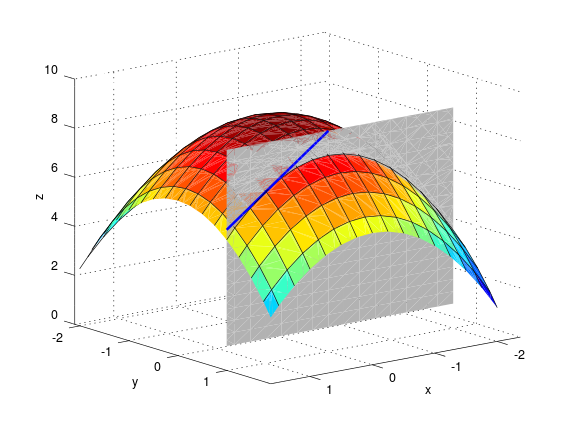
\includegraphics[width=1\linewidth]{xpart.png}
            \caption*{Snertivigur við skurðferil sléttunnar \\ $y=b$ og yfirborðsins $z = f(x,y)$ \\ í punktinum $(a,b,f(a,b))$ er \\ $\mathbf{T}_1 = (1,0,f_1(a,b))$.}
        \end{minipage}%
        \begin{minipage}{\textwidth}
            \centering
            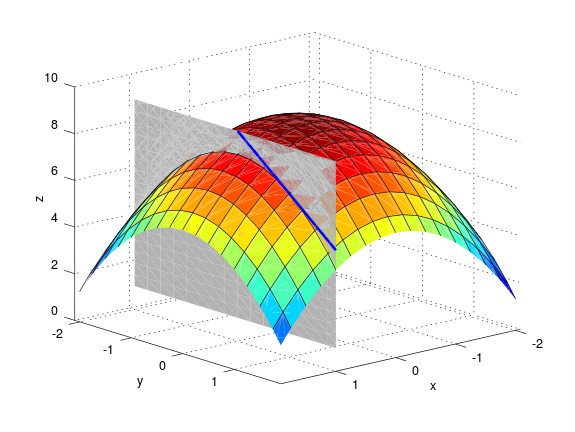
\includegraphics[width=1\linewidth]{ypart.png}
            \caption*{Snertivigur við skurðferil sléttunnar \\ $x=a$ og yfirborðsins $z = f(x,y)$ \\ í punktinum $(a,b,f(a,b))$ er \\ $\mathbf{T}_2 = (0,1,f_2(a,b))$.}
        \end{minipage}
\end{figure}
 
\begin{enumerate}
    \item 
  Látum $\rv: D\subseteq \R^2\rightarrow \R^3$ vera stikaflöt.  
Ef $(x_0, y_0, z_0)=\rv(u_0, v_0)$ er punktur á fletinum sem 
$\rv(u,v)=\big(x(u,v), y(u,v), z(u,v)\big)$ stikar og
föllin $x(u,v), y(u,v), z(u,v)$ eru diffranleg í punktinum $(x_0,
y_0)$ þá er vigurinn
     $$\nv =\frac{\partial \rv}{\partial u}\times 
\frac{\partial \rv}{\partial v}$$
reiknaður með $u=u_0$ og $v=v_0$ þvervigur á flötinn í punktinum 
$(x_0, y_0, z_0)$.
\end{enumerate}
 


\subsubsection{Skilgreining  \rtask{}}
Ef vigrarnir $\frac{\partial \rv}{\partial u}(u,v)$ og $\frac{\partial \rv}{\partial v}(u,v)$ eru óháðir
fyrir alla punkta $(u,v)\in D$ þá er sagt að stikunin sé {\em
  regluleg}. 

 

\subsubsection{Athugasemd \rtask{}}
Ef vigrarnir  
$\frac{\partial \rv}{\partial u}(u_0,v_0)$ og $\frac{\partial\rv}{\partial v}(u_0,v_0)$ eru óháðir þá spanna þeir snertiplan við
flötinn í punktinum $\rv(u_0,v_0)$. Snertiplanið hefur stikun 

$$\Pi(u,v) = \rv(u_0,v_0)+u\frac{\partial \rv}{\partial u}(u_0,v_0)
+v\frac{\partial \rv}{\partial v}(u_0,v_0).$$






\subsection{Flatarheildi} 

\subsubsection{Verkefni  \rtask{}}
\begin {enumerate}
 \item Flatarmál flata -- sambærilegt við bogalengd ferla.  
\item Heildi falls yfir flöt með tilliti til flatarmáls -- sambærilegt við heildi falls eftir ferli með tilliti til bogalengdar.
\item Heildi vigursviðs yfir flöt -- svipar til heildis vigursviðs eftir ferli. 
 \end {enumerate}









\subsection{Flatarmál flata} 

\subsubsection{Skilgreining  \rtask{}}
  Látum $\rv:D\rightarrow \R^2$ vera
reglulegan stikaflöt sem stikar flöt $\cal S$.  Flatarmál $\cal S$ er  
$$ A=\tvint_D\,dS=\tvint_D \big|{\textstyle\frac{\partial \rv}{\partial u}
\times\frac{\partial \rv}{\partial v}}\big|\,dudv.$$



\subsubsection{Formúla  \rtask{}}
Látum $f(x,y)$ vera diffranlegt fall skilgreint á
mengi $D$ í $\R^2$.  Flatarmál grafsins $z=f(x,y)$ er gefið með
formúlunni 
$$A=\tvint_D dS=\tvint_D {\textstyle\sqrt{1+
\big(\frac{\partial f}{\partial x}\big)^2+
\big(\frac{\partial f}{\partial y}\big)^2}}\,\,dx\,dy.$$
   



\subsection{Flatarheildi} 

\subsubsection{Verkefni  \rtask{}}
\begin {enumerate}
 \item Flatarmál flata -- sambærilegt við bogalengd ferla.  
\item Heildi falls yfir flöt með tilliti til flatarmáls -- sambærilegt við heildi falls eftir ferli með tilliti til bogalengdar.
\item Heildi vigursviðs yfir flöt -- svipar til heildis vigursviðs eftir ferli. 
 \end {enumerate}


\subsubsection{Skilgreining \rtask{}}
  Látum $\rv:D\rightarrow \R^3$ vera
reglulegan stikaflöt sem stikar flöt $\cal S$.  Flatarmál $\cal S$ er  
$$ A=\tvint_D\,dS=\tvint_D \big|{\textstyle\frac{\partial \rv}{\partial u}
\times\frac{\partial \rv}{\partial v}}\big|\,dudv.$$




\subsubsection{Formúla \rtask{}}
 Látum $f(x,y)$ vera diffranlegt fall skilgreint á
mengi $D$ í $\R^2$.  Flatarmál grafsins $z=f(x,y)$ er gefið með
formúlunni 
$$A=\tvint_D dS=\tvint_D {\textstyle\sqrt{1+
\big(\frac{\partial f}{\partial x}\big)^2+
\big(\frac{\partial f}{\partial y}\big)^2}}\,\,dx\,dy.$$



\subsubsection{Formúlur \rtask{form}}

 Ritum $dS$ fyrir flatarmálselement á fleti $\cal S$.  
\begin{itemize}
\item Ef $\rv:D\subseteq\R^2\rightarrow \R^3$ er stikun á $\cal S$ þá
  er $$dS=\bigg|\frac{\partial \rv}{\partial u}\times\frac{\partial
  \rv}{\partial v}\bigg|\,du\,dv.$$
\item Ef $\cal S$ er graf $z=g(x,y)$ þá er 
$$dS=\sqrt{1+g_1(x,y)^2+g_2(x,y)^2}\,dx\,dy.$$


\end{itemize}


 Ritum $dS$ fyrir flatarmálselement á fleti $\cal S$.  
\begin{itemize}
\item Gerum ráð fyrir að flöturinn $\cal S$ í $\R^3$ hafi þann eiginleika að
  ofanvarp hans á $xy$-planið sé eintækt eða með öðrum orðum hægt er
  að lýsa fletinum sem grafi $z=f(x,y)$.
Ef $\nv$ er þvervigur á
flötinn og $\gamma$ er hornið sem þvervigurinn $\nv$ myndar við
jákvæða hluta $z$-ássins þá er 
$$dS=\bigg|\frac{1}{\cos\gamma}\bigg|\,dx\,dy
=\frac{|\nv|}{|\nv\cdot\kv|}\,dx\,dy.$$

Í þessu tilviki gildir einnig að ef $\cal S$ er lýst sem 
hæðarfleti $G(x,y,z)=C$ þá er 
$$dS=\bigg|\frac{\nabla G(x,y,z)}{G_3(x,y,z)}\bigg|\,dx\,dy.$$
\end{itemize}






\subsubsection{Skilgreining \rtask{}}
 Látum $\rv: D\rightarrow \R^3$ vera
reglulega stikun á fleti $\cal S$.   
Heildi falls $f(x,y,z)$ yfir flötinn $\cal S$ með tilliti til flatarmáls er
$$\tvint_{\cal S} f\,dS=\tvint_D f(\rv(u,v)) \big|{\textstyle\frac{\partial
    \rv}{\partial u} 
\times\frac{\partial \rv}{\partial v}}\big|\,dudv.$$



\subsection{Einingarþvervigrasvið} 

\subsubsection{Skilgreining \rtask{}}

Látum $\cal S$ vera flöt í $\R^3$.  {\em Einingarþvervigur} $\nv$ á flötinn
$\cal S$ í punktinum $P$ er einingarvigur hornréttur á
snertiplan við flötinn í punktinum $P$.  

{\em Einingarþvervigrasvið} á
$\cal S$ er samfellt vigursvið $\Nv$ sem er skilgreint í öllum punktum
$\cal S$ þannig að fyrir $(x,y,z)\in{\cal S}$ er vigurinn $\nv(x,y,z)$
einingarvigur sem er hornréttur á snertiplan við flötinn í punktinum
$(x,y,z)$.

\begin {figure}[h!]
 \centering
            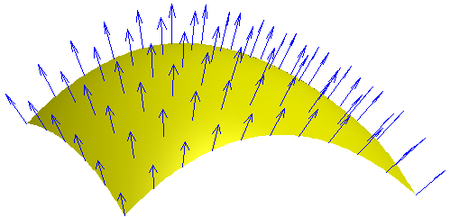
\includegraphics[width=0.65\linewidth]{normalfield.png}
            \caption*{}
\end {figure}




\subsection{Áttanlegir fletir} 

\subsubsection{Skilgreining \rtask{}}

Flöturinn $\cal S$ er sagður {\em áttanlegur} ef til er einingarþvervigrasvið
$\Nv$ á $\cal S$.  

\medskip
{\em Áttun} á áttanlegum fleti felst í því að velja annað af tveimur
mögulegum einingaþvervigrasviðum. 


\begin {figure}[h!]
 \centering
            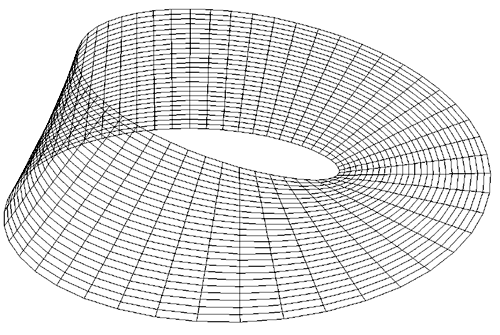
\includegraphics[width=0.40\linewidth]{mobius.png}
            \caption*{Möbiusarborði er ekki áttanlegur.}
\end {figure}

 \subsubsection{Umræða \rtask{}}
  Ef áttanlegur flötur $\cal S$ hefur jaðar þá skilgreinir áttunin stefnu á jaðri $\cal S$. Venjan er að velja stefnu jaðarsins þannig að þegar gengið er eftir honum sé einingarþvervigrasviðið á vinstri hönd (hægri handar regla).
  
  \bigskip
  Ef tveir áttanlegir fletir hafa jaðar má splæsa þeim saman í áttanlegan flöt með því að líma þá saman á (hluta af) jöðrunum og gæta þess að jaðrarnir hafi andstæða stefnu á samskeytunum.
 

\begin {figure}[h!]
 \centering
            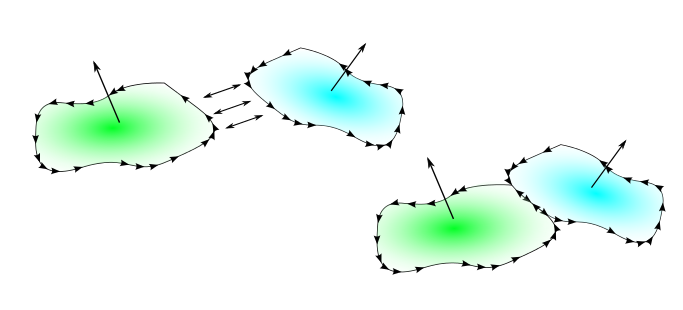
\includegraphics[width=0.95\linewidth]{joinsurf.png}
            \caption*{}
\end {figure}



\subsubsection{Setning \rtask{attun}}
 Gerum ráð fyrir að $\cal S$ sé áttanlegur
flötur og $\rv:D\subseteq\R^2\rightarrow \R^3$ sé regluleg stikun á
$\cal S$ (það er, $\frac{\partial \rv}{\partial u}$ og
$\frac{\partial \rv}{\partial v}$ eru samfelld föll af $u$ og $v$ og 
vigrarnir $\frac{\partial \rv}{\partial u}$ og
$\frac{\partial \rv}{\partial v}$ eru línulega óháðir).
Þá er 
$$\Nv=
\frac{\frac{\partial \rv}{\partial u}\times\frac{\partial
    \rv}{\partial v}}
{|\frac{\partial \rv}{\partial u}\times\frac{\partial
    \rv}{\partial v}|}$$
einingarþvervigrasvið á $\cal S$.  




\subsection{Heildi vigursviðs yfir flöt - Flæði} 

\subsubsection{Skilgreining og ritháttur \rtask{}}
 Látum $\cal S$ vera áttanlegan flöt stikaðan
af reglulegum stikaferli  $\rv:D\subseteq\R^2\rightarrow \R^3$ með
samfelldar hlutafleiður.  Látum $\Nv$ tákna einingarþver\-vigrasviðið
sem gefið er í \ref{attun}.  Heildi vigursviðs $\Fv$ yfir flötinn $\cal S$ er
skilgreint sem 
$$\tvint_{\cal S} \Fv\cdot\Nv\,dS
=\tvint_D \Fv(\rv(u,v))\cdot \bigg(
\frac{\partial \rv}{\partial u}\times\frac{\partial \rv}{\partial
  v}\bigg)\,
du\,dv.$$
Slík heildi eru oft nefnd \emph{flæði vigursviðsins} $\Fv$ {\em gegnum flötinn} $\cal S$.

\bigskip
 Ritum $d\Sv=\Nv\,dS$.  Þá  er 
$$\tvint_{\cal S} \Fv\cdot\Nv\,dS=\tvint_{\cal S} \Fv\cdot\,d\Sv.$$



\subsubsection{Samantekt \rtask{}}
  
\begin{enumerate}
\item Ef $\rv:D\subseteq\R^2\rightarrow \R^3$ er stikun á $\cal S$ þá
  er $$d\Sv=\pm \bigg(\frac{\partial \rv}{\partial u}\times\frac{\partial
  \rv}{\partial v}\bigg)\,du\,dv.$$
\item Ef $\cal S$ er graf $z=f(x,y)$ þá er 
$$d\Sv=\pm\bigg(-\frac{\partial f}{\partial x},-\frac{\partial
  f}{\partial y},1\bigg)\,dx\,dy.$$
\item Gerum ráð fyrir að flöturinn $\cal S$ í $\R^3$ hafi þann eiginleika að
  ofanvarp hans á $xy$-planið sé eintækt eða með öðrum orðum hægt er
  að lýsa fletinum sem grafi $z=f(x,y)$.
Ef fletinum $\cal S$ er lýst sem 
hæðarfleti $G(x,y,z)=C$ þá er  
$$d\Sv=\pm\frac{\nabla G(x,y,z)}{|\nabla G(x,y,z)|}\,dS=
\pm\frac{\nabla G(x,y,z)}{G_3(x,y,z)}\,dx\,dy.$$
\end{enumerate}
Val á áttun felst í því að velja $+$ eða $-$ í formúlunum hér að
ofan.  





\subsubsection{Túlkun \rtask{}}
 Hugsum okkur að vigursviðið $\Fv$ lýsi streymi
vökva.  Hugsum svo flötinn $\cal S$ sem himnu sem vökvinn getur
streymt í gegnum.  Áttun á $\cal S$ gefur okkur leið til að tala um
hliðar flatarins og að vökvinn streymi í gegnum flötinn frá
einni hlið til annarrar.  Streymi vökvans gegnum flötinn (rúmmál per
tímaeiningu) er gefið með heildinu $\tvint_{\cal S} \Fv\cdot\Nv\,dS$
  þar sem streymi í stefnu $\Nv$ reiknast jákvætt.

\begin {figure}[h!]
 \centering
            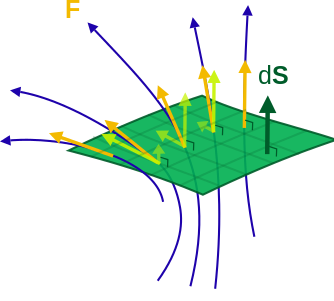
\includegraphics[width=0.45\linewidth]{flux.png}
            \caption*{}
\end {figure}



\end{document}
